\documentclass[
  final,
  portrait,
  paperwidth=150cm,
  paperheight=200cm,
  margin=3cm   % margen externo del póster
]{baposter}



% Tamaños
\renewcommand{\normalsize}{\fontsize{17pt}{17pt}\selectfont}
\renewcommand{\small}{\fontsize{14pt}{15pt}\selectfont}
\renewcommand{\footnotesize}{\fontsize{12pt}{14pt}\selectfont}
\renewcommand{\scriptsize}{\fontsize{11.5pt}{11.5pt}\selectfont}

\usepackage{fontspec}
\usepackage{amsfonts}
\usepackage{graphicx}
\usepackage{units}
\usepackage{xfrac}

\setmainfont{EB Garamond}[
    Ligatures=TeX,
    UprightFont = * Regular,
    ItalicFont = * Italic,
    BoldFont = * SemiBold,
    BoldItalicFont = * SemiBold Italic,
]
\setsansfont{EB Garamond}[
    Ligatures=TeX,
    UprightFont = * Regular,
    ItalicFont = * Italic,
    BoldFont = * SemiBold,
    BoldItalicFont = * SemiBold Italic,
]

\selectcolormodel{cmyk}

\graphicspath{{figures/}} % Directory in which figures are stored

\newcommand{\compresslist}{%
\setlength{\itemsep}{0pt}%
\setlength{\parskip}{1pt}%
\setlength{\parsep}{0pt}%
}

\begin{document}

\definecolor{Mycolor2}{HTML}{001c3f}  % E35205 % Pantone 166 C - naranja intenso
\definecolor{Mycolor1}{HTML}{1B4D3E} % Verde árbol oscuro
\definecolor{bgColorOne}{HTML}{F5F3F3} % Gris muy claro, cálido, fondo general
\definecolor{boxColorOne}{HTML}{E0E1E5} % Gris claro un poco más oscuro, fondo de cajas

\begin{poster}
% ================== OPCIONES ==================
{
grid=false,
headerborder=none,
colspacing=.7em,
bgColorOne=bgColorOne,
bgColorTwo=bgColorOne,
borderColor=Mycolor1,
headerColorOne=Mycolor2,
headerColorTwo=Mycolor2,
headerFontColor=white,
boxColorOne=boxColorOne,
textborder=none,
eyecatcher=true,        % <— SIN logo a la izquierda
headerheight=0.081\textheight,  % un poco más alto para que respire
headershape=rounded,
headershade=plain,
headerfont=\Large\textsf,
linewidth=2pt
}
% =============== 1) EYE-CATCHER ===============
{}
% ================== 2) TÍTULO Y AUTORES =================
{
\bfseries\fontsize{50}{48}\selectfont
Estimación de riesgo latente en el mercado de EE. UU.\\mediante variables representativas \\[0.3em]
\Large Heriberto Espino Montelongo \quad $\bullet$ \quad Owen Paredes Conde \quad $\bullet$ \quad Pedro José García Guevara
}
% 
% ================== 3) LOGOS ==================
{}

% Ahora sí, empiezan las cajas del póster:
\headerbox{\LARGE{\textbf{Introducción}}}{name=introduction,column=0,row=0, span=2}{
\vspace{0.15cm}

La identificación de episodios de \textbf{riesgo estructural} en los mercados financieros es
fundamental para el análisis macrofinanciero y la gestión de riesgos. En particular, variables
asociadas al desplazamiento hacia \textbf{activos seguros} y al \textbf{estrés financiero global}
contienen información relevante sobre cambios en el régimen de riesgo, aunque dicha señal
no suele observarse de manera directa.

\medskip

En este trabajo proponemos un \textbf{índice de riesgo latente} \(R_t\) construido a partir de
señales financieras globales, como el \textbf{precio del oro}, el \textbf{tipo de cambio del dólar},
la \textbf{volatilidad implícita} y los \textbf{diferenciales de crédito corporativo}. Estas variables
se combinan mediante un \textbf{Modelo de Factores Dinámicos (MFD)} para extraer un
componente común que represente la evolución subyacente del riesgo sistémico.

\medskip

Posteriormente, estimamos la tendencia estructural \(\hat{\tau}_t\) mediante
\textbf{Mínimos Cuadrados Penalizados}, donde el parámetro de suavizamiento se selecciona
con el \textbf{índice de suavidad} de Guerrero (2007) a través de un enfoque numérico con
conjuntos de validación. Esto permite una calibración más objetiva de la relación señal--ruido
y una mejor evaluación de cambios estructurales en el riesgo implícito. Así, el resultado es
un indicador interpretable y estadísticamente fundamentado para el monitoreo del riesgo en
el mercado de bonos del Tesoro de los Estados Unidos.

\vspace{0.1cm}
}

\headerbox{\LARGE{\textbf{Definiciones}}}{name=Definiciones,column=2,row=0,span=1}{
\vspace{0.1cm}
\small

\textbf{Modelo de Factores Dinámicos (DFM).}
Sea \(X_t=(X_{1t},\dots,X_{nt})'\) el vector de variables financieras observadas. Un DFM
supone que su comovimiento puede resumirse mediante un número reducido de
\textbf{factores latentes} \(f_t\), de forma que
\[
X_t = \Lambda f_t + e_t,
\]
donde \(\Lambda\) es la matriz de cargas factoriales y \(e_t\) recoge los componentes
idiosincráticos. La dinámica temporal del sistema se incorpora modelando \(f_t\) como un
proceso estocástico, lo que permite extraer una señal común asociada al
\textbf{riesgo sistémico subyacente}. En este trabajo, el índice \(R_t\) se interpreta como una
medida latente construida a partir de dicho componente común \cite{StockWatson2011}.

\medskip

\textbf{Suavizamiento por Mínimos Cuadrados Penalizados.}
Una vez construido \(R_t\), su tendencia estructural \(\tau_t\) se estima resolviendo
\[
\min_{\{\tau_t\}}
\sum_{t=1}^{N}(R_t-\tau_t)^2
+
\lambda \sum_{t=d+1}^{N}(\nabla^d \tau_t - m)^2,
\]
donde el primer término ajusta la tendencia a los datos y el segundo penaliza la falta de
suavidad. El parámetro \(\lambda>0\) controla el equilibrio entre ajuste y suavizamiento:
valores pequeños producen una tendencia más flexible, mientras que valores grandes generan
una trayectoria más suave \cite{Guerrero2007}.

\medskip

\textbf{Índice de suavidad de Guerrero.}
Guerrero (2007) propone seleccionar \(\lambda\) a partir de un \textbf{índice de suavidad}
\(S_d(\lambda,N)\), que mide la proporción de suavidad inducida por la penalización.
En lugar de fijar directamente \(\lambda\), primero se establece un nivel deseado de suavidad
y luego se obtiene el valor de \(\lambda\) que lo reproduce numéricamente. En este trabajo,
esa búsqueda se complementa con \textbf{conjuntos de validación}, eligiendo el valor de
\(\lambda\) que minimiza el error de pronóstico fuera de muestra. Esto permite una selección
más objetiva de la relación señal--ruido y reduce el sesgo en los extremos de la muestra
\cite{Guerrero2007}.
\vspace{0.144cm}

}
\headerbox{\LARGE{\textbf{Metodología}}}{name=methodology,column=0,below=introduction,span=2}{
\vspace{0.1cm}
\begin{enumerate}
    \item \textbf{Recopilación y preprocesamiento:} Extraer las series de tiempo de alta frecuencia (VIX, WTI, Spreads de crédito y Curva de Rendimientos) desde bases de datos como FRED y Stooq.
    \item \textbf{Modelo de Factores Dinámicos (DFM):} Estimar un DFM para extraer un factor latente común que resuma el co-movimiento y la dinámica subyacente de las variables financieras y macroeconómicas.
    \item \textbf{Transformación y Suavizamiento:} Aplicar el \textbf{método de Guerrero} para encontrar el parámetro óptimo de transformación que estabilice el ruido del índice.
    \item \textbf{Validación y Optimización:} Calibrar los hiperparámetros del modelo seleccionando los valores óptimos mediante la evaluación del error de pronóstico en un \textbf{set de validación} aislado.
    \item \textbf{Análisis de Comportamiento:} Analizar la evolución temporal del índice resultante para identificar regímenes de estrés financiero, puntos de inflexión y su relación con ciclos macroeconómicos.
\end{enumerate}
}

\headerbox{\LARGE{\textbf{Resultados}}}{name=result,column=0,span=3,below=methodology}{

\begin{minipage}[t]{0.45\linewidth}
\vspace{0pt}
\centering

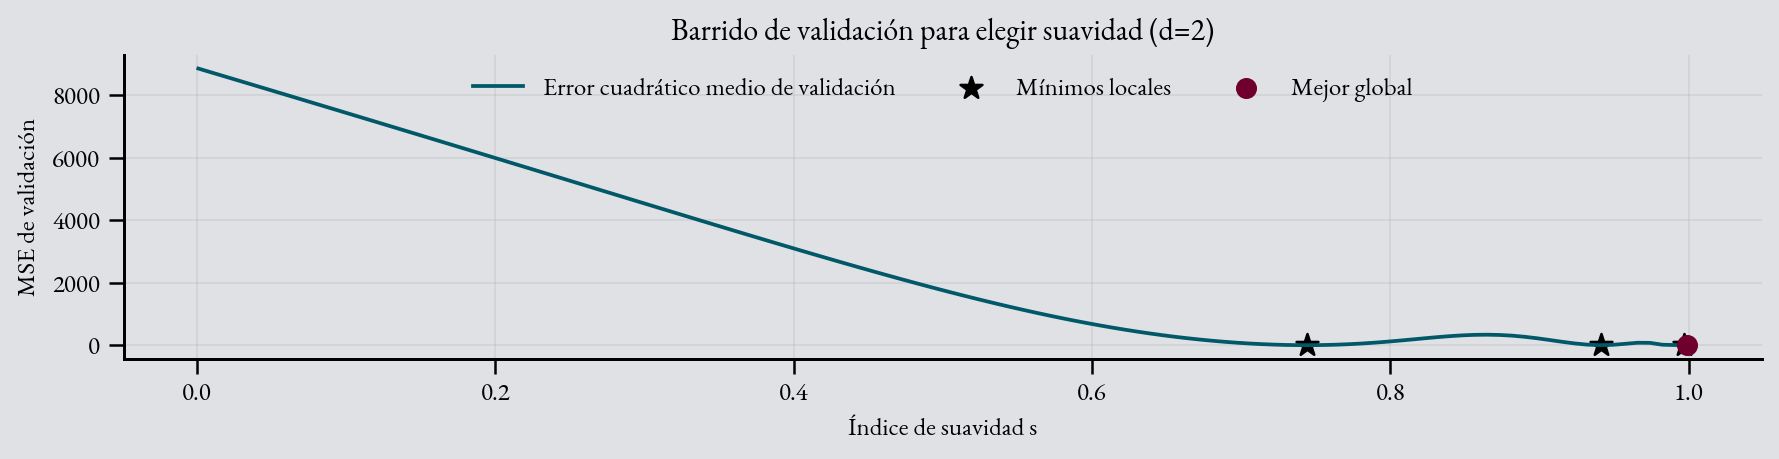
\includegraphics[width=1\linewidth]{validation_scan.PNG}

{\scriptsize (a) Factor vs series transformadas}

\vspace{0.6em}

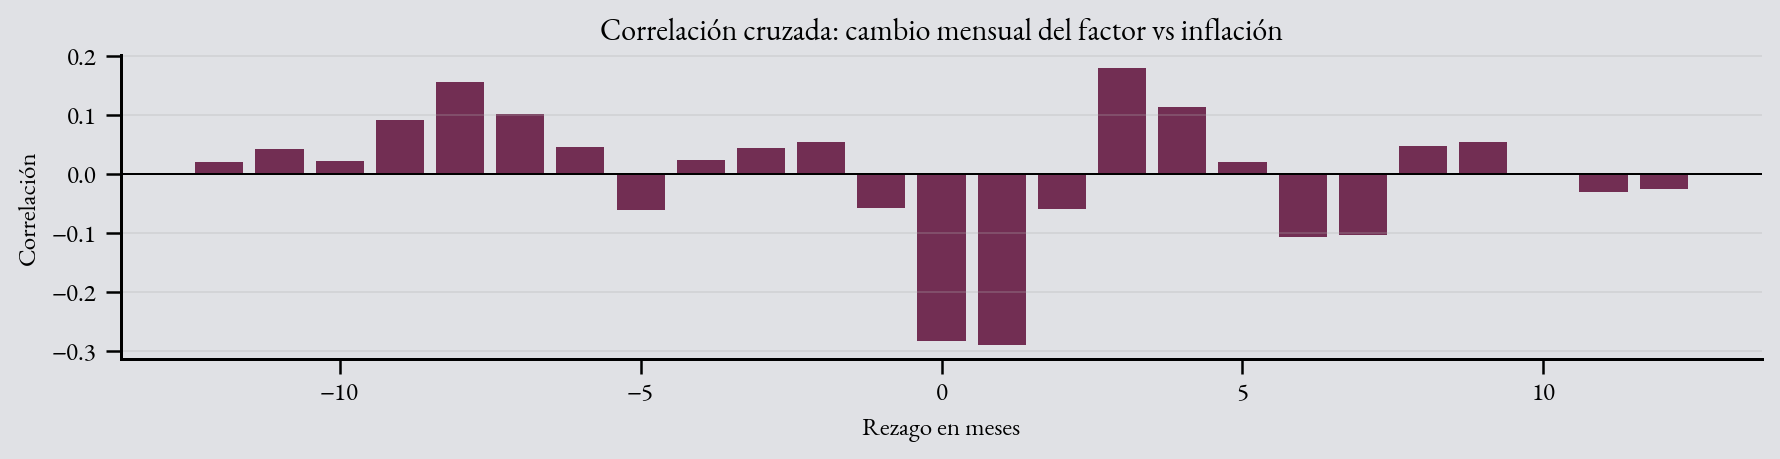
\includegraphics[width=1\linewidth]{cross_correlation.PNG}

{\scriptsize (b) Factor vs series transformadas}

\vspace{0.6em}

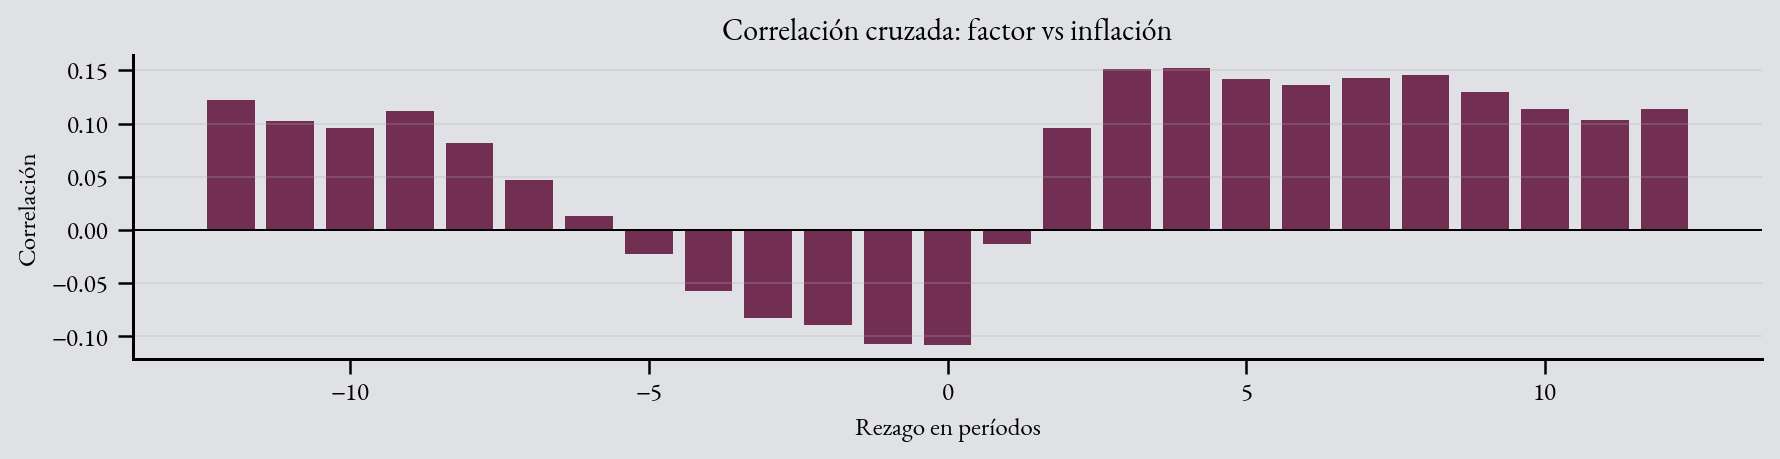
\includegraphics[width=1\linewidth]{factor_inflation_cross_correlation.PNG}

{\scriptsize (c) Factor vs series transformadas}

\end{minipage}
\hfill
\begin{minipage}[t]{0.50\linewidth}
\vspace{0pt}
\centering

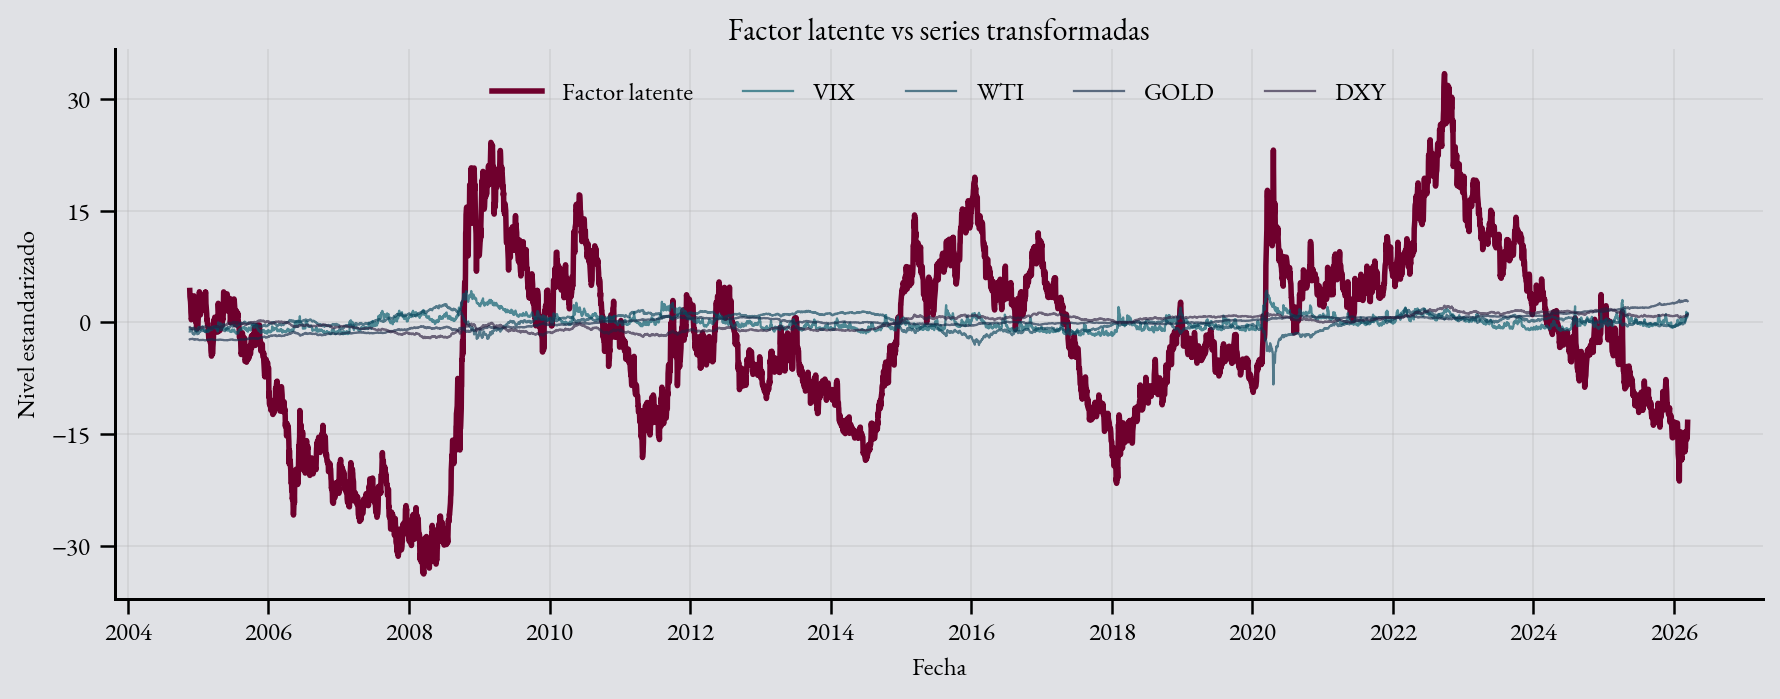
\includegraphics[width=\linewidth]{factor_vs_series_transformadas.PNG}

{\scriptsize (d) Factor vs series transformadas}

\vspace{1em}

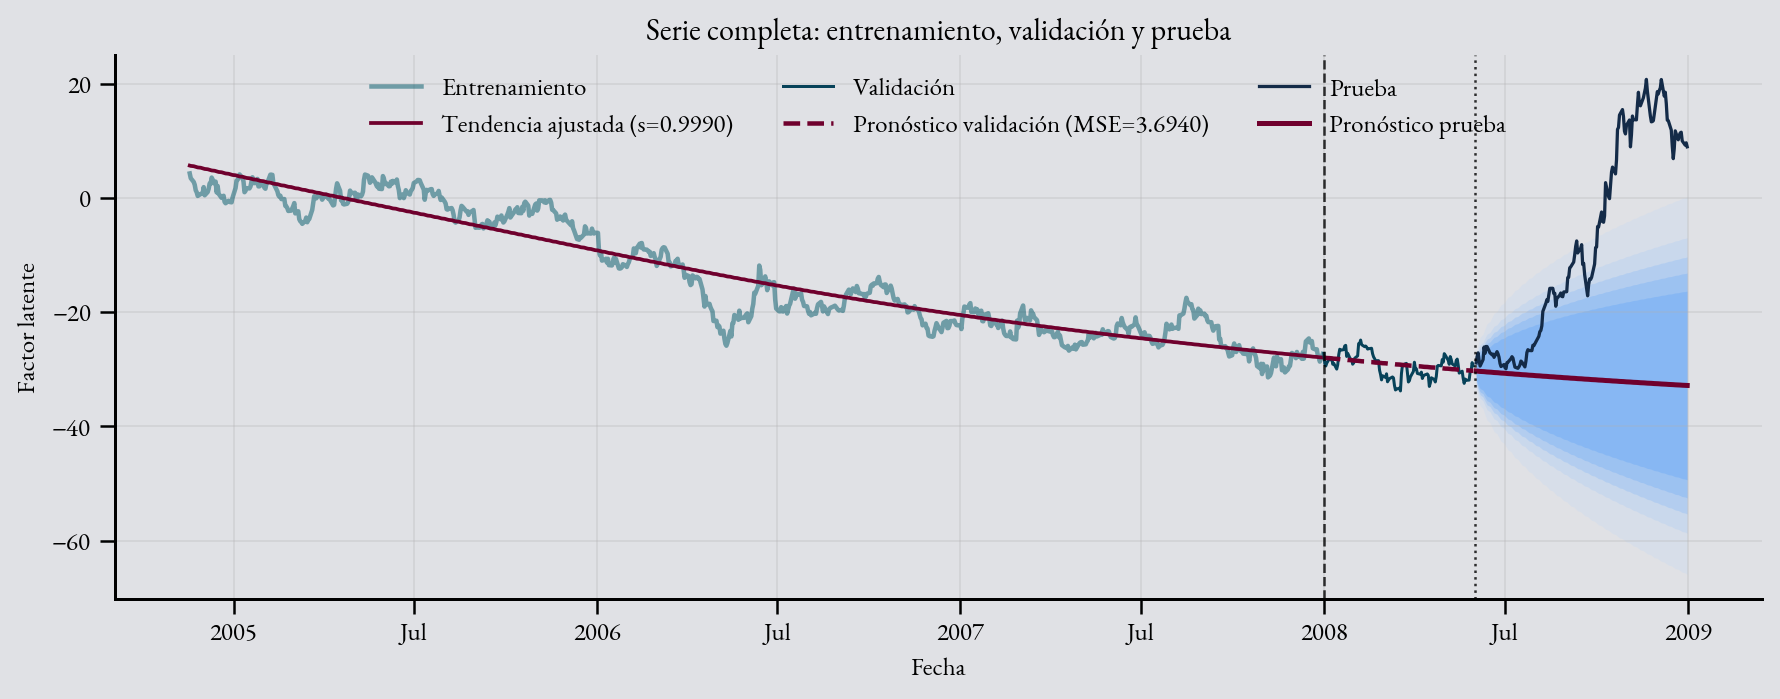
\includegraphics[width=\linewidth]{full_timeline_train_validation_test.PNG}

{\scriptsize (e) Factor vs series transformadas}

\end{minipage}

}

\headerbox{\LARGE{\textbf{Conclusiones y Trabajo Futuro}}}{name=conclusion,column=0,below=result,span=2,above=bottom}{

\vspace{0.1cm}
\begin{itemize}
    \item El \textbf{Modelo de Factores Dinámicos (DFM)} permitió sintetizar exitosamente las variables de riesgo y tasas de interés en un único indicador, capturando el co-movimiento subyacente del mercado.
    \item La aplicación del \textbf{método de Guerrero} fue fundamental para optimizar el \textit{smoothing index}, reduciendo el ruido estocástico de las series de alta frecuencia sin perder la sensibilidad a los cambios de régimen.
    \item La evaluación del hiperparámetro óptimo en el \textbf{set de validación} confirmó que el modelo es robusto fuera de la muestra, evitando el sobreajuste a las crisis históricas.
    \item Se identificaron claramente los periodos de estrés financiero, demostrando que el índice reacciona de manera coherente ante choques macroeconómicos.
    \item Queda como trabajo posterior hacer una prueba retrospectiva (\textit{backtesting}) para evaluar la rentabilidad y utilidad del índice como señal de alerta temprana en estrategias de asignación de activos o cobertura de portafolios.
\end{itemize}
\vspace{.1cm}

}

\headerbox{\LARGE{\textbf{Referencias}}}{name=references,column=2,below=result,span=1}{
\renewcommand{\refname}{} 
\vspace{-0.3cm} 
\scriptsize
\begin{thebibliography}{99}\compresslist

\bibitem{Guerrero2007}
V. M. Guerrero. Time series smoothing by penalized least squares.
\textit{Statistics \& Probability Letters}, 77(12), 1225--1234, 2007.

\bibitem{StockWatson2011}
J. H. Stock \& M. W. Watson. Dynamic factor models.
\textit{Oxford Handbook of Economic Forecasting}, Oxford University Press, 2011.

\bibitem{BaurLucey2010}
D. G. Baur \& B. M. Lucey. Is gold a hedge or a safe haven? An analysis of stocks, bonds and gold.
\textit{Financial Review}, 45(2), 217--229, 2010.

\end{thebibliography}
}

\headerbox{\LARGE{\textbf{Contacto}}}{name=qr,column=2,below=references,span=1,above=bottom}{

\begin{center}

\begin{minipage}{0.30\linewidth}
\centering

\includegraphics[width=0.95\linewidth]{QR_Heriberto.png}\\
\scriptsize Heriberto Espino M.
\end{minipage}
\hfill
\begin{minipage}{0.30\linewidth}
\centering

\includegraphics[width=0.95\linewidth]{QR_Owen.png}\\
\scriptsize Owen Paredes Conde
\end{minipage}
\hfill
\begin{minipage}{0.30\linewidth}
\centering

\includegraphics[width=0.95\linewidth]{QR_Pedro.png}\\
\scriptsize Pedro J. García Guevara
\end{minipage}

\end{center}


}


\end{poster}

\end{document}
